
\chapter{Application}
For PPI AG, the goal is to use the research conducted during this Master thesis as a scientific basis for a future application of this technology in one of their own business use cases. Therefore, this chapter will assess, whether emotion recognition is a viable assistance for consultants, as well as customers in the selected use case of video-call consultations.
\newline\newline
Firstly, a prototype was developed to prove that emotion recognition is a viable option for real-time predictions from a webcam stream. Secondly, a more meaningful interpretation of emotions was needed to provide consultants or customers with a more actionable metric. Interest was chosen to be the metric used to identify a customer's intention. Thus, an user experiment was conducted that compares the predicted interest based on emotions recognized from facial expressions with the stated level of interest by participants.

%%%%%%%%%%%%%%%%%%%%%%%%%%%%%%%%%%%%%%%%%%%%%%%%%%%%%%%%%%%%
\section{Prototype}
The first prototype was constructed as a local application that takes its video input from the PC's webcam. When the user presses the 'SPACE' key, the program extracts the current frame of the video stream, detects the human face, recognizes its emotion in terms of valence and arousal, and prints the results onto the screen. A snapshot of this is provided in the following figure \ref{fig:PrototypeRealTime}. 

\begin{figure}[H]
  \begin{center}
  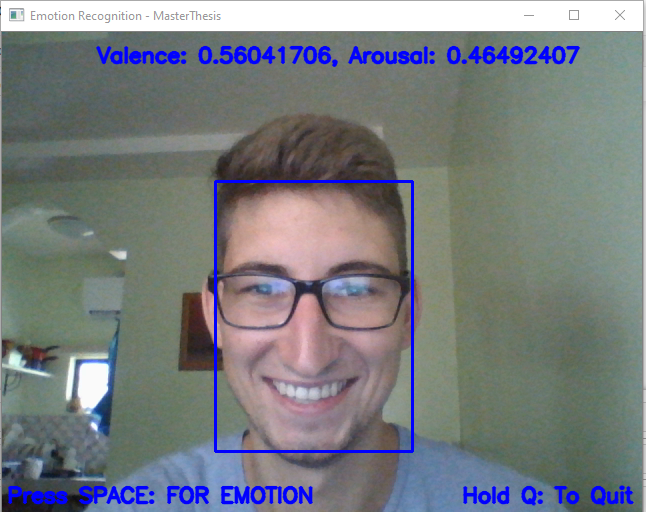
\includegraphics[angle=0, width=0.8\textwidth]{Figures/webcam_foto.PNG}
  \caption{The prototype application allows to recognize emotions in terms of valence and arousal in real-time.}
  \label{fig:PrototypeRealTime}
  \end{center}
\end{figure}

\textbf{Landmarks}\newline
It was from special interest to PPI AG whether such an approach would be suitable for real-time usage, especially in regards to utilizing landmarks. 
\newline\newline
A small test of 10 probes indicated that it took on average 0.7 seconds to perform emotion recognition without any landmarks in production. In comparison to that, additionally detecting landmarks with the dlib shape predictor \citep{Kazemi:2014:ShapePredictor} and feeding them into the model did not result in any delay, as it also took on average 0.7 seconds. Such a low number, with less than 1 second, proves that this approach is definitely suitable for real-time use cases. 
\newline\newline
However, it needs to be pointed out that this could only be achieved with the dlib shape predictor, unlike an Active Appearance Model which would likely need more time to be constructed. Furthermore, it is to be expected that the average duration of 0.7 seconds further decreases when taking into account that the prediction be performed on a powerful server with GPU support instead of a laptop computer.

%%%%%%%%%%%%%%%%%%%%%%%%%%%%%%%%%%%%%%%%%%%%%%%%%%%%%%%%%%%%
\section{User Experiment (Interest)}
The experiment provided further insights into the utilization of emotion recognition for the identification of human interest. Thus, the goal was to be able to draw conclusions about the suspected correlation between recognized emotions and human interest. Before diving into the design and outcomes of the experiment, an identification approach of interest had to be created based upon current literature.
\newline\newline
There herein presented approach for identifying interest was based on the ideas from two different scientific contributions:
\begin{itemize}
    \item \citet{Kamaruddin:2016:MeasuringCustomerSatisfaction} determined a level of interest/appreciation by measuring how positive or negative an emotion (= valence) experience was on average.
    \item \citet{Poirier:2016:AdsFacialExpression} measured the effectiveness of ads by analyzing facial expressions. They claimed that the emotional journey is the strongest predictor of ad appreciation which is why they focused on the curve/profile created by the predicted emotion values for valence.
\end{itemize}

% \citet{Poirier:2016:AdsFacialExpression} measured the effectiveness of ads by analyzing facial expressions. \citet{Poirier:2016:AdsFacialExpression} claimed that the emotional journey is the strongest predictor of ad appreciation. The researchers predicted the emotional values for valence and arousal, and focused at the curve/profile created by values for valence. The researchers' assumption seemed to be that a certain profile of the valence curve is the main determinant of whether an ad was successful. While this sounds promising, it also raises the question of whether these ad appreciation in commercial ads also converts into actual positive ratings, or even product sales

% Even though their actual interval duration is not known, the FaceReader \citep{Noldus:2020:Facereader} application, a commercial solution that was tested during this Master thesis, already offers a calculation for 'Interest' that was based on a interval length of 2 seconds. Moreover, \citet{Kamaruddin:2016:MeasuringCustomerSatisfaction} introduced a threshold for determining a neutral emotion category.

Inspired by these approaches, the prototype application imitates some of this behaviour and based its 'Interest' measurement solely on valence. For each frame extracted every second from the video stream, valence is predicted. Interest was calculated by averaging the predicted values of valence for the last 5 frames.
% If the value of valence is below the threshold of -0.2 it is counted as 'negative', if it is above +0.2 it is counted as 'positive' and if it is inside those two threshold values it is regarded as 'neutral'. Depending on ratio of the number of emotions that were classified as 'positive' vs 'negative', the 'Interest' is determined with a range from 0 to +1.
% \newline\newline
% \textbf{Example calculation:}

% \begin{table}[H]
% \begin{center}
% \begin{tabular}{@{}cccl@{}}
% \toprule
% Image & Valence & Classif. & \multicolumn{1}{c}{Interest calculation} \\ \midrule
% \#1 & -0.58 & negative &  \\
% \#2 & -0.24 & negative &  \\
% \#3 & 0.00 & neutral & neutral is not considered \\
% \#4 & 0.17 & neutral & neutral is not considered \\
% \#5 & 0.36 & positive &  \\
% \begin{tabular}[c]{@{}c@{}}...\\ (up to 20)\end{tabular} & ... & ... &  \\
% \multicolumn{1}{l}{} & \multicolumn{1}{l}{} & \begin{tabular}[c]{@{}c@{}}COUNT:\\ 2x negative\\ 1x positive\end{tabular} & \begin{tabular}[c]{@{}l@{}}= (\#pos * 100) / (\#pos + \#neg)\\ = (1 * 100) / (1 + 2) = 33.3\end{tabular} \\ \bottomrule
% \end{tabular}
% \caption{Example: Interest Calculation}
% \label{tab:InterestCalculation}
% \end{center}
% \end{table}

% In the table \ref{tab:InterestCalculation} an example calculation for Interest is presented. It starts with taking the last 20 frames/images taken (in this case only 5 are presented for illustration reasons). The Valence of these frames is predicted and subsequently classified as negative, neutral or positive depending on the threshold of -0.2 and +0.2. Afterwards, the number of frames classified are counted and the Interest is calculated with the following formula: (\#positive * 100)/(\#positive + \#negative). Thus, the result in the presented example is 33.33.


%%%%%%%%%%%%%%%%%%%%%%%%%%%%%%%%%%%%%%%%%%%%%%%%%%%%%%%%%%%%%%%%%%

\subsection{Experiment design}
The goal of this experiment is to compare the test person's perceived subjective interest with the interest predicted by the before mentioned approach. In order to make this experiment objective and comparable between different participants, it was chosen that instead of direct interaction, participants get to watch commercial ads. Through these ads it was expected to get the objectivel comparable results which are still somewhat similar to real-life video calls, for example during a product presentation.
\newline\newline
For the analysis of the participants interest, the webcam video stream was needed to be recorded exactly at the same time when the video was played. Additionally, a mechanism had to be devised to calculate a level of interest from the recognized emotions. For this, an experiment had to be implemented that could be given to participants, and that allows them to indicate their own current level of interest.
\newline\newline
For such an implementation there were multiple considerations about the setup type. The possible options are presented in the following table, where a 'X' indicates the non-fulfillment of an indispensable quality of an setup, while '/' indicates a constraint and ':)' indicates that the quality is fully fulfilled by the setup.

\begin{table}[H]
\begin{center}
\begin{tabular}{cccccc}
\hline
\textbf{} & Effort & \begin{tabular}[c]{@{}c@{}}Web-Cam\\ Video\end{tabular} & \begin{tabular}[c]{@{}c@{}}Continuous\\ interest rating\end{tabular} & \begin{tabular}[c]{@{}c@{}}Easily\\ deployable\end{tabular} & \begin{tabular}[c]{@{}c@{}}Results\\ retrievable\end{tabular} \\ \hline
\textbf{\begin{tabular}[c]{@{}c@{}}Questionnaire\\ (e.g. w/ Google Forms)\end{tabular}} & low & {\color[HTML]{FE0000} \textbf{X}} & {\color[HTML]{FE0000} \textbf{X}} & {\color[HTML]{32CB00} \textbf{:)}} & {\color[HTML]{32CB00} \textbf{:)}} \\
\textbf{\begin{tabular}[c]{@{}c@{}}Advanced survey tool\\ (e.g. w/ Phonic)\end{tabular}} & low & {\color[HTML]{32CB00} \textbf{:)}} & {\color[HTML]{FE0000} \textbf{X}} & {\color[HTML]{32CB00} \textbf{:)}} & {\color[HTML]{FFC702} \textbf{/}} \\
\textbf{\begin{tabular}[c]{@{}c@{}}Packaged Local Appl.\\ (e.g. w/ Python)\end{tabular}} & high & {\color[HTML]{32CB00} \textbf{:)}} & {\color[HTML]{32CB00} \textbf{:)}} & {\color[HTML]{FE0000} \textbf{X}} & {\color[HTML]{FFC702} \textbf{/}} \\
\textbf{\begin{tabular}[c]{@{}c@{}}Web-based Server Appl.\\ (e.g. w/ PythonAnywhere)\end{tabular}} & high & {\color[HTML]{FE0000} \textbf{X}} & {\color[HTML]{32CB00} \textbf{:)}} & {\color[HTML]{32CB00} \textbf{:)}} & {\color[HTML]{32CB00} \textbf{:)}} \\
\textbf{\begin{tabular}[c]{@{}c@{}}Web-based Client Appl.\\ (e.g. w/ ReactJS)\end{tabular}} & high & {\color[HTML]{32CB00} \textbf{:)}} & {\color[HTML]{32CB00} \textbf{:)}} & {\color[HTML]{32CB00} \textbf{:)}} & {\color[HTML]{FFC702} \textbf{/}} \\ \hline
\end{tabular}
\caption{Implementing a web-based frontend application with ReactJS was the favorite choice for conducting a user experiment.}
\label{tab:appExperiment}
\end{center}
\end{table}

The setups mentioned in table \ref{tab:appExperiment} were verified from top to bottom. First, the questionnaire and survey tools were investigated, because they, on the one hand, allowed for a quick implementation, but also did not allow room for the required customization to conduct this experiment. A locally-run, stand-alone application would have accommodated all of this. However, due to its nature and size, it would be difficult to provide the participants with the program needed for the experiment and to retrieve its results. The best choice identified in this work was to develop a web-based application.
\newline\newline
A web-based server application hosted by PythonEverywhere would have fulfilled all the requirements, however, hooking onto participants’ webcams did not prove to be possible. As a result, it was decided to develop a browser-based standalone web-application with ReactJS. It allowed for the needed customization and only posed a constraint in terms of results retrieval (the participants had to download the results and send them manually back).
\newline\newline
The user interface for the developed application is comprised of the presented video to be watched by the participant, as well as another smaller video that captures and records the webcam of the participant. There is also a slider for the indication of the current interest level of the participant, as well as a 'Start', 'Stop' and 'Download' button. The following figure shows the default screen when accessing the web page:

\begin{center}
\begin{figure}[H]
  \begin{center}
  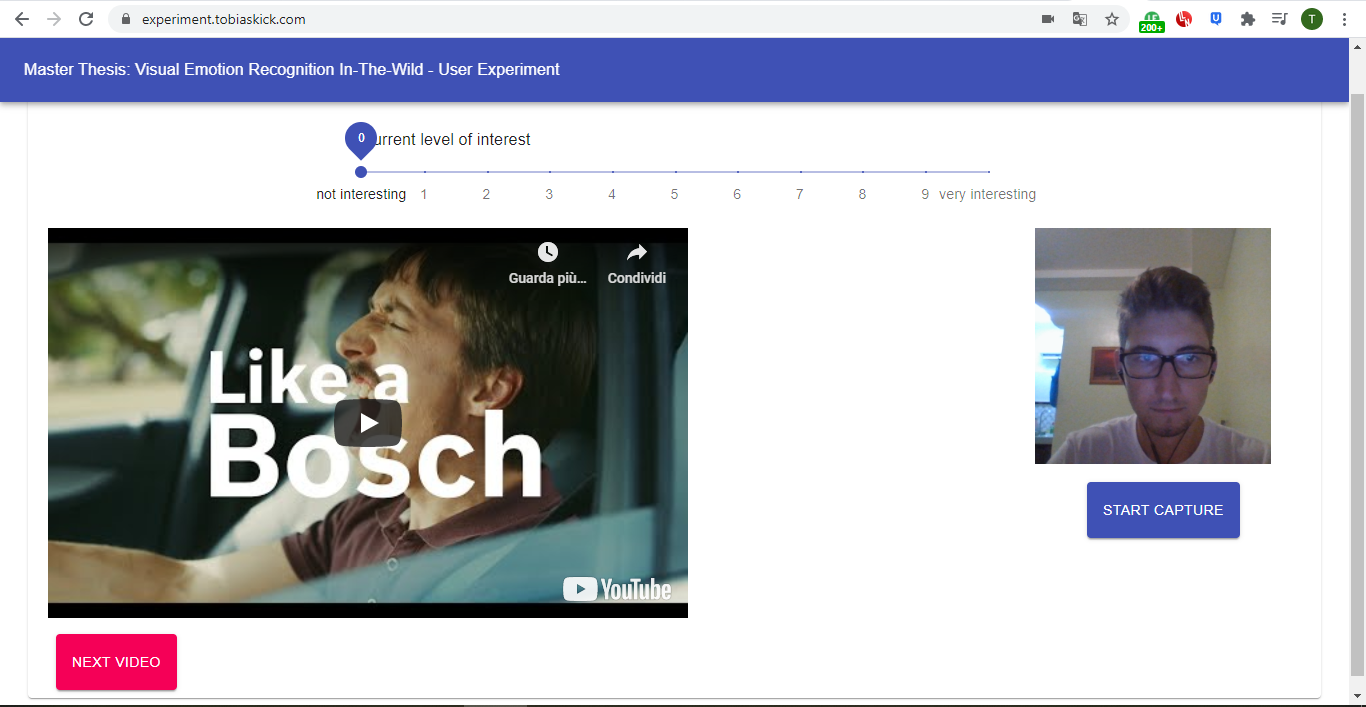
\includegraphics[angle=0, width=1.0\textwidth]{Figures/UserExperiment.PNG}
  \caption{The experiment's user interface allows to watch commercials, while it captures at the same time the webcam stream, and allows the user to continuously indicate the current level of interest.}
  \label{fig:InterfaceUserExperiment}
  \end{center}
\end{figure}
\end{center}

There are three video clips from YouTube embedded into the web page. These video clips are successful commercial ads that are supposed to induce a moderate range of emotions in participants.
\newline\newline
For participants to watch those video clips and indicate their currently experienced level of interest, they had to follow the following instructions:

\begin{enumerate}[noitemsep]
    \item Open the website: experiment.tobiaskick.com
    \item Make sure your laptop/PC camera is not blocked and works
    \item In case of a pop-up: Allow the usage of your camera
    \item Make sure you can see yourself in the small rectangular box on the right-hand side
    \item Start the video with a click on 'Start Capture'. This will also activate the recording of your face.
    \item Watch the video and simultaneously indicate your current level of interest by setting the slider on the appropriate level (from 0 to +10)
    \item Adjust your interest continuously. You can pause and resume the video/recording.
    \item When video finished: Download results by clicking on 'Download results'
    \item In case of a pop-up: Allow the download of multiple files at the same time. It should download one .csv file and a .webm file
    \item Go on to the next video by clicking on the button 'Next video'
    \item Start the same process again for the next video by clicking the button 'Start Capture'
    \item Finally, send the results, consisting of a *.webm and *.csv file for each video clip, back to tkick93@gmail.com (totalling 6 files). Alternatively, drop the files in the following Google Driver folder (link was attached) and indicate your name.
\end{enumerate}

After the participant conducted all these tasks, a *.webm and *.csv file was received for each video. The *.webm files had to be converted to MP4 with an Online Converter (frame rate of 24 per second). After that the VLC media player was used to filter frames so that it returned a frame for each second of the video.
\newline\newline
In the next step, these frames were read into a Python program that predicted the values for valence and arousal for each frame and calculated a measure of interest based on the previously presented approach. The results were then compared to the stated interest in the *.csv file.


\subsection{Experiment outcomes}
The goal of the experiment was to compare the indicated level of interest of all participants with a calculated value of interest which was based on predictions from the proposed model architecture in this thesis.
\newline\newline
Due to different video conditions between participant's web camera, as well as the discrepancy between discretely stated interest by participants and continuously predicted interest, the model is not expected to be able to match the subjectively stated level of interest exactly. However, the underlying hypothesis is that there exists a trend between subjectively stated interest and continuously predicted interest, even though the magnitude might be different.
\newline\newline
This hypothesis was tested by calculating the Pearson Correlation between the interest stated by participants and the interest predicted with emotion recognition. An average was calculated over the correlation measure of all participants. 
\newline\newline
Generally speaking, a Pearson Correlation between 0.3 and 0.5 is regarded as a low correlation, between 0.5 and 0.7 as moderate correlation and above 0.7 as high correlation. In order to make the claim that emotional valence is a reliable indicator for human interest, the goal was to achieve at least a correlation of 0.5.
\newline\newline
The metric for the experiment is the average Pearson correlation. The gathered data includes three presented video clips for each of the 10 participants (participants with invalid data were not considered here). The best solution without cross validation achieved in this experiment on average a Pearson correlation of 0.12. This number indicates a positive, but very weak correlation. Due to such a weak correlation it cannot be excluded whether the results were just achieved by chance. This is why for this experiment is regarded as not being able to prove any meaningful correlation between emotional valence and the actual interest indicated by participants.
\newline\newline
Next to the actual result, the experiment gave way to further insights:\newline
\begin{itemize}
    \item \textbf{Emotional valence:} The emotional valence predicted by the neural network is not varying much throughout the participants. However, the magnitude of valence is slightly different for each participant. This might indicate that the expression of emotions is really low during the experiment of watching commercial ads, which in turn makes it very hard for the network to differentiate facial expressions. This is an interesting insight, as this would probably also be the case during real-life video calls.
    \item \textbf{Time required for interest identification:} A sample taken during the analysis revealed that loading all the components for the neural network to be constructed took 3 minutes and 44 seconds. After the model was loaded, the actual prediction of emotions and interest calculation was performed which took 2 minutes and 8 seconds for 84 analyzed frames. This translates into 1.52 seconds per frame that are needed on average to predict an emotion and to identify the corresponding interest (The analysis was conducted on a fairly standard laptop with a Intel Core i5-5200U CPU processor).
\end{itemize}

% \textbf{Viability in real-time video calls}
% especially focus on the time aspect for detecting the bounding box + landmark detection/shape model construction.

% Comparison dlib's shape model vs. Active Appearance Model
% \begin{quote}
%     The dlib 'Face Landmark Detection' algorithm is blazing fast, in fact it takes about 1–3ms (on desktop platform) to detect (align) a set of 68 landmarks on a given face.
% \end{quote} 
% https://medium.com/datadriveninvestor/training-alternative-dlib-shape-predictor-models-using-python-d1d8f8bd9f5c

% @InProceedings{Kazemi_2014_CVPR,
% author = {Kazemi, Vahid and Sullivan, Josephine},
% title = {One Millisecond Face Alignment with an Ensemble of Regression Trees},
% booktitle = {Proceedings of the IEEE Conference on Computer Vision and Pattern Recognition (CVPR)},
% month = {June},
% year = {2014}
% }
